\section{Introduction}
\emph{I was 34 minutes late to lecture due to misunderstanding the start time - thanks to Kalpak for providing his notes!}

\subsection{Probabilities in Statistical Mechanics}
In stat mech, probabilities are given by:
\begin{equation}
    P(\mu) = \frac{e^{-\beta H(\mu)}}{Z}
\end{equation}
for a microstate $\mu$. Here, $Z$ is the partition function:
\begin{equation}
    Z = \sum_\mu e^{-\beta H(\mu)}
\end{equation}
and $\beta = \frac{1}{k_B T}$ is the inverse temperature. The free energy can be obtained as:
\begin{equation}
    F = -\frac{1}{\beta}\ln Z
\end{equation}

What is meant by a state $\mu$? In some sense, there is a tension, as one slices up the continuous state space of classical physics. This is resolved by fields.

\subsection{Spin Models}
A rich setting to explore statistical mechanics is spin models. For example, the celebrated \emph{Ising model}is defined by the Hamiltonian:
\begin{equation}
    H_{\text{Ising}} = \sum_{ij}J_{ij}S_iS_j
\end{equation}
with $J_{ij}$ the coupling between classical spins $S_i \in \set{1, -1}$. We can also generalize this for arbitrary spin directions by promoting the spins to vectors (giving rise to a continuous degree of freedom), yielding the Heisenberg model:
\begin{equation}
    H_{\text{Heisenberg}} = \sum_{ij}J_{ij}\v{S}_i \cdot \v{S}_j.
\end{equation}

As is clear from the sums appearing in the above expressions, we are considering discrete spins (perhaps on some lattice). We can convert to momentum space via a Fourier transform, and then via a ``coarse-graining procedure'' (formalized by the renormalization group) we obtain a roughly continuous spectrum, which we may treat as a field.

\subsection{From discrete models to fields}
For example, we can consider the linear dispersion relation:
\begin{equation}
    \omega(k) = c\abs{k}
\end{equation}
which gives rise to the density of states:
\begin{equation}
    d^3n = u(k)d^3k = u(\omega)d\omega
\end{equation}
Which by then considering a sphere in $k$-space of surface area $4\pi k^2$ this becomes:
\begin{equation}
    qu(\omega) = u(k)4\pi k^2 \frac{dk}{d\omega}
\end{equation}
The energy density $u(k)$ we take to be constant, i.e. just $V/(2\pi)^d = L^3/(2\pi)^d$ (for a box of length $L$) and $\dod{k}{\omega}$ is obtained from the dispersion relation, yielding:
\begin{equation}
    d^3n = \frac{L^3}{2\pi^2}\frac{\omega^2}{c^3}
\end{equation}
This is the Rayleigh argument for black-body radiation. Of course this is incorrect, as the density of energy diverges as $\omega \to \infty$. This is fixed by quantum mechanics, where the Einstein blackbody argument yields:
\begin{equation}
    u(\nu) = \frac{8\pi h\nu^3}{c^3}\frac{1}{e^{\frac{h\nu}{k_B T}} - 1}.
\end{equation}

Let's now return to the spin model, and consider a field construction of the system. We define te magnetization:
\begin{equation}
    m = \sum_{i=1}^N S_i
\end{equation}
and we nwo coarse grain, taking $m = m(x)$ to be a function of $x$. We look at a window/block of spins and describe it with a theory in the continuum limit. For a given window/block $i$, we can consider:
\begin{equation}
    m(x_i) = \sum_{i, j < N} S_{i+j}
\end{equation}

Phenomenologically, we can guess the theory with legal terms:
\begin{equation}\label{eq:GinzLandau}
    H = \int dx \left[am^2(x) + bm^3(x) + cm^4(x) + k(\nabla m)^2 + k'(\nabla^2 m)^2 + \ldots \right]
\end{equation}
and use this to probe the explore of the system. Note that the Hamiltonian cannot have terms of order $m$ or $\Delta m$ as this breaks the $\mathbb{Z}_2$ inversion symmetry. However, such terms can enter in the forms of external fields (yielding terms like $hm$) which break the symmetry.

\subsection{Phase Transitions}

We can also think about phases of matter and phase transitions between them. E.g. phase transition between solid/liquid/gas phases are discontinuous. Can have discontinuous phase transitions between different phases; find free energy minimums of two different phases, and they cross. There's a subtlety at the critical point, however, which we return to later (it turns out that this point is scale invariant, and described by a conformal field theory). Also note that there are $V$ for which no apparent symmetries broken in the liquid-to-gas transition, i.e. the phase transition is continuous (but it does turn out that an emergent symmetry becomes broken).

\begin{figure}[htbp!]
    \centering
    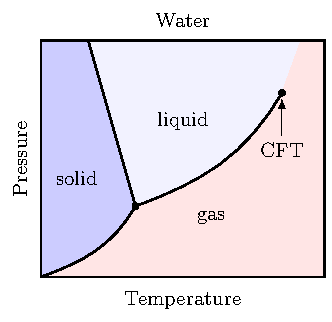
\includegraphics[]{Lectures/Figures/PT_diagram.pdf}
    \caption{Phase diagram of water. There is a lot of rich phenomenology in the phase transitions, for example at the critical point where the system is scale invariant and described by a CFT.}
    \label{fig:PTwater}
\end{figure}

In the magnet case, we can have magnetic and non-magnetic phase. In magnetic phase, has to choose a direction for the magnetization to point in. This breaks the $\ZZ_2$ symmetry. Looking at the phase diagram for a magnet, we have the parameters $T$ temperature and $h$ the external magnetic field. For $h > 0$ we have magnetization up and for $h < 0$ we have magnetization down. At zero temperature the transition is abrupt. There is a critical temperature $T_c$ above which the transition is smooth, and below $T_c$ we have varying degrees of an abrupt transition. Interestingly, the critical point between liquid and gas ``looks like'' an Ising transition.

\begin{figure}[htbp!]
    \centering
    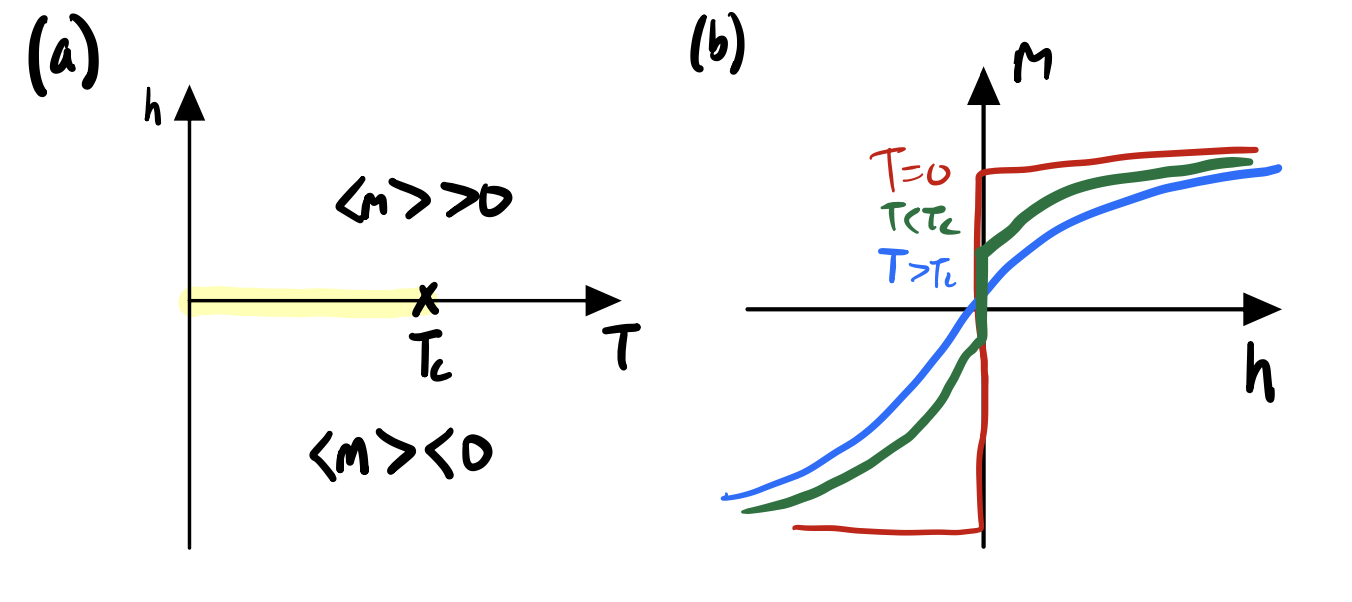
\includegraphics[scale=0.55]{Lectures/Figures/Ising_phases.png}
    \caption{(a)$h$ (external field) vs. $T$ (temperature) phase diagram for the Ising model and (b) behaviour of $m$ (magnetization) as a function of $h$ for different $T$. For $h > 0$ we have $\avg{m} > 0$ and vise versa for $h < 0$. For $T < T_c$, there is an abrupt transition in $m$ at $h=0$ (yellow line). This can be seen by studying the behaviour of $m$ for different temperatures; for $T = 0$ the transition is abrupt (as we would expect; since the external field is the only contribution to the energy, any finite magnetic field fully polarizes the spins). Below $T_c$ the transition stays abrupt, though with a smaller ``jump'' in the magnetization, and above $T_c$ the transition is smooth.}
    \label{fig:Ising_phases}
\end{figure}

We can obtain scaling laws for the magnetization:
\begin{equation}
    m(T, h = 0) = \begin{cases} 0 & T > T_c \\ \abs{t}^\beta & T< T_c \end{cases}
\end{equation}
\begin{equation}
    m(T = T_c, h) \sim h^{1/\delta}
\end{equation}

There are other quantities we may compute; for example we could measure the magnetic susceptibility $\chi = \dpd{m}{h}(t)$. Because the system becomes very polarizable near the phase transition, we may expect that $\chi$ has a peak/divergence at $T = T_c$, which is characterized by a further exponent. We could also compute the specific heat of the system, which also has its associated exponent and so on.

There's a whole zoo of critical exponents, and it turns out that there are (universality) classes where the exponents are the same - i.e. near these phase transitions very different systems are governed by the same theories.

Note that the theory described by Eq. \eqref{eq:GinzLandau} is known as Ginzburg-Landau theory (or the \emph{mean-field} theory), and was written down to describe phenomenology. We have a power series expansion in the magnetization, with the coefficients (e.g. $a$) as smooth functions governed by $T, h$, and so on.

We can consider a $\phi^4$ theory:
\begin{equation}
    F = a\phi^2 + b\phi^4 + h\phi
\end{equation}
with a phenomenological guess of $a = a_0(T - T_c)$.
\begin{equation}
    \dod{F}{\phi} = 0, \quad \phi^2 = -\frac{a}{b} \text{ or } \phi = 0
\end{equation}
We then have $\phi \sim (T_c - T)^{1/2}$, i.e. $\beta = 1/2$.

General procedure: Start with mean field theory. Then, aspects of field theory will turn out. One aspect will be thermal fluctuations about the mean field theory states. Then we think about terms like $k(\nabla m)^2$, which tells us that there are energy costs to (e.g.) mis-aligned spins. This is known still as the Gaussian model as the Hamiltonian with this term is still quadratic in the fields. The moment I have a gradient term, I get modes in the system that can propagate. If I have a lot of modes, I don't get a phase transition.

Scaling Hypothesis - I know there are a set of critical exponents. How are they related? Via scaling. So, suppose I look at the system on different scales. As I average over different scales, if the system has to look self-similar. RG gives us a way to obtain critical exponents.

Other systems - we will also look at systems in low-dimensions, which can be interesting. There are also systems with inherent disorder/randomness, e.g. glasses which are frozen but not ordered systems. There is at least one model that realizes this, which Parisi got a Nobel for. We will also look at dynamical systems; what happens to open/driven systems? There are ways to formally write them in a very similar language. E.g. friction, forced flow, growing things at an interface, biology. Finally, we may study information and data. The straightforwards introduction for physicists is spin glasses, which can (in theory) be used to encode data via learning a set of interactions $J_{ij}$. 